\documentclass[twocolumn, a4paper]{jsarticle}
\usepackage[top=20truemm,bottom=20truemm,left=20truemm,right=20truemm]{geometry}
\usepackage[dvipdfmx]{graphicx,color}
\usepackage{cite}
\usepackage{url}

\setlength{\columnsep}{5mm}

\begin{document}
\title{情報システム工学演習II 画像処理 レポートテンプレート}
\author{08D12345 大倉 史生}
\date{20xx年x月x日} 
\twocolumn[
\maketitle
]

これは、情報システム工学演習II 画像処理演習のレポートテンプレートである。
\begin{itemize}
\item 本レポートの作成には\LaTeX を使うことを推奨するが、必須ではない。他の方法でレポートを書く場合も、本テンプレートのレイアウトを参考にすると良い。
\item ページ数は、本レイアウトを使う場合、参考文献リストを除いて1~2ページ程度を目安とする(が、それより長くても良い)。日本語か英語で記述すること。
\item 実装したアプリの内容をうまくアピールするように、本レポートのタイトルを適切に変更すること。
\item かきあげたレポートをコンパイルし、\{学籍番号\}.pdfのファイル名で提出すること。その際、この辺のインストラクション用の文章は削除すること。
\end{itemize}
本演習は、アプリの「独創性」および「完成度」、レポート記述の「充実度」で評価する。
下記に章立ての一例を示すが、この内容・順番にこだわる必要はない。

\section{背景}
皆さんの生活にどのような問題があり、この演習で作ったシステム、ツール、アプリがどのように役に立つか説明すること。

あなた自身、あるいは特定のターゲットとなるユーザにとっての実用性がきちんと説明されていれば十分である。
一般的な観点では実用的でなくとも、あなた自身(あるいは特定のユーザ)が有用であると思い得ることがレポートの記述からわかれば、それで良い。
例えば、「暇つぶし」や「楽しい」などもすごく立派な用途である。これらがとなり得るシナリオをレポート中にしっかり記載すること。

\section{実装したツール}
本演習で実装したツールの概要を以下に示す。

\subsection{外部仕様}
ユーザはどのようにそのツールを使うのか記述する。どんな画像を用意して、何を起動する、どのボタンを押す、そうすると何が得られる、など。

\subsection{内部仕様}
そのツールは、どのような仕様で実装されたか説明する。処理のフローなどを示すのも有用。参考にした資料がある場合は引用すること(論文の引用例\cite{canny}、URLでの引用例\cite{material})。

\subsection{使用した関数やライブラリ・実行環境}
デフォルト以外のライブラリを使った場合、また、特殊な環境で実行することを前提とする場合は記載すること。


\section{実行例}
実行例を記載すること。実際の入出力画像を貼り付けるのも有用であるが、どのような結果が得られるのかを文章でも説明することが重要。
図\ref{fig:ou}に図の例を示す。

\begin{figure}[t]
\centering

\includegraphics[width=\linewidth]{ou.png}
\caption{図の例}
\label{fig:ou}
\end{figure}

\section{考察・感想}
考察や感想を記載する。

\begin{thebibliography}{99}
\bibitem{canny} John Canny. A computational approach to edge detection. {\em IEEE Transactions on Pattern Analysis and Machine Intelligence},  No.~6, pp. 679--698, 1986.
\bibitem{material} 情報システム工学演習II画像処理 演習資料, \url{https://github.com/fumio125/enshu_ip}.
\end{thebibliography}


\begin{figure}[t]
\centering
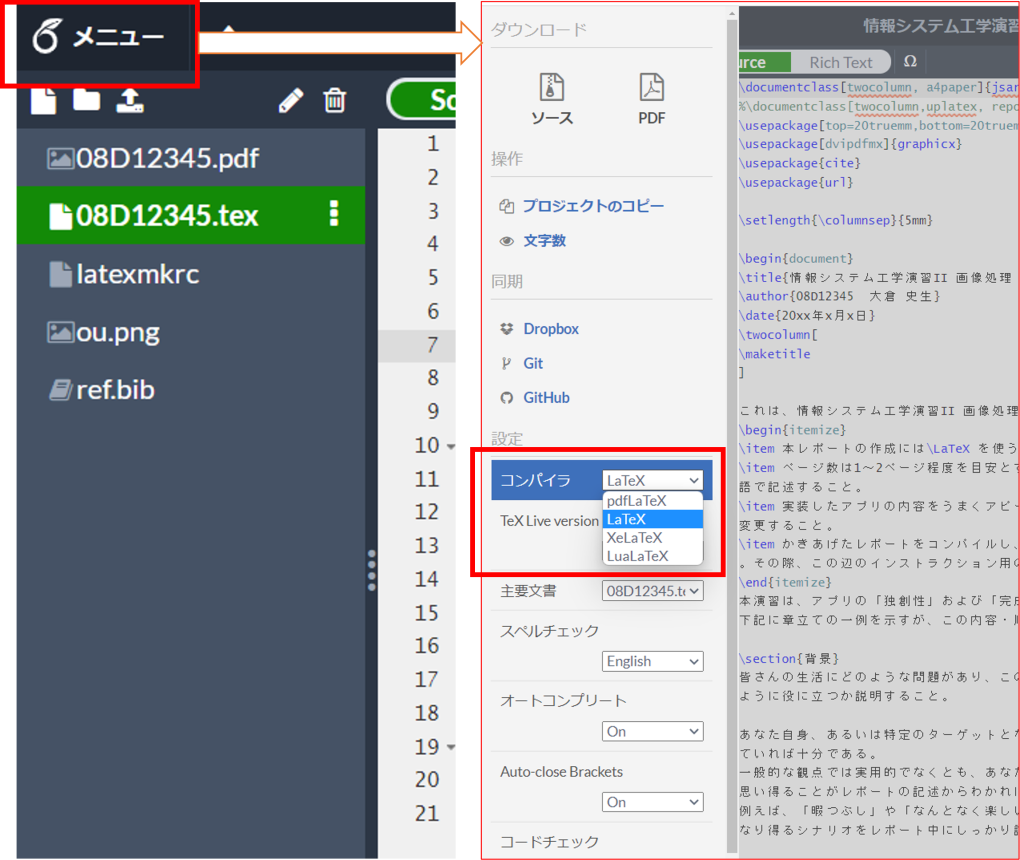
\includegraphics[width=\linewidth]{overleaf.png}
\caption{Overleafの設定}
\label{fig:overleaf}
\end{figure}

\section*{Appendix: \LaTeX 環境構築}
\subsection*{クラウドツール}
Overleaf\footnote{Overleaf, \url{https://ja.overleaf.com/}}などのクラウドツール使うと、手元の環境構築が必要ないため便利。\texttt{report}フォルダをzip圧縮して、「プロジェクトのアップロード」をすると編集できる。
日本語の文書のコンパイルには、図\ref{fig:overleaf}に示すような設定変更が必要であり、メニューから、コンパイラをLaTeXに変更してコンパイルすると良い。
なお、必要な項目を記載した\texttt{latexmkrc}も用意する必要があるが、すでに\texttt{report}フォルダ内に含まれているので改めて追加する必要はない。

\subsection*{自前環境}
手元に環境構築する場合はTeX Live\footnote{Tex Live, \url{https://www.tug.org/texlive/}}を使うと良い。インストール方法は\TeX WikiのTeX Liveのページ\footnote{\TeX Wiki, \url{https://texwiki.texjp.org/?TeX%20Live}}が詳しい。 
日本語の文章なので、pLaTeX(など)でコンパイルすること。また、参考文献のコンパイルにはpBibTeXを使う。

TeX Liveと一緒にインストールされる編集ソフト(TeXworks)を使う場合、図\ref{fig:texworks}のようにコンパイルツールをpLaTeXにすると良い(「再生ボタン」あるいはWindowsの場合はCtrl+Tでコンパイルできる)。
参考文献と本文中の文献番号、図表の番号などを対応付けるためには、何回か走らせる(本文中の?が消えるまで;普通は2回で良い)必要がある。

\begin{figure}[t]
\centering
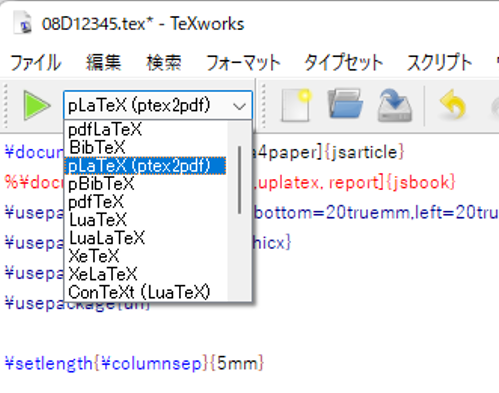
\includegraphics[width=\linewidth]{texworks.png}
\caption{TeXworksの設定}
\label{fig:texworks}
\end{figure}


\end{document}